\documentclass[12pt,onecolumn,titlepage]{article}
% using the aztechreport package fixes lots of stuff about the formatting,
% title page, etc.
\usepackage{azacademicreport}
\usepackage{graphicx}
\usepackage{amssymb}
\usepackage{xspace}
\usepackage{float}
\usepackage[table,xcdraw]{xcolor}

\graphicspath{ {Pics/}}

% You can create new commands, as below, which are useful to  have
% for this, or other, tex files. I just re-create them when i need them.
\newcommand{\figureref}[1]{Fig.~\ref{#1}}
\newcommand{\sectionref}[1]{Section~\ref{#1}}

% You can create commands just to use for this file, too
\newcommand{\tex}{\TeX\xspace}
\newcommand{\latex}{\LaTeX\xspace}
\newcommand{\miktex}{MiK\tex}
\newcommand{\wys}{\protect{WYSIWYG}\xspace}
\newcommand{\file}[1]{\texttt{#1}}
\newcommand{\cmd}[1]{\texttt{\%\ #1}\xspace}
\newcommand{\Filename}{templateUniversal\xspace}

\begin{document}


\title{Gas Station Finder:\\Project Design Document}
\shorttitle{Project Design Document}

% comment out this line, if a single-user submission (like a term report)
%\teamname{IfApplicable}

\author[au1]{Zheng Li(zhengli233@email.arizona.edu)} 
\author[au2]{Kejia Li(jacob1230@email.arizona.edu)} 
\author[au3]{Harish Kumar Kothari, Abhishek(abhishek09@email.arizona.edu)}
		

%\author[a2]{Student Number Two (email2@ece.arizona.edu)}

%\author[au3]{Student von~Lastname, III (email3@ece.arizona.edu)}

\course{ECE573--Software Engineering Concepts}
\term{Spring 2017}
\faculty{Matt Bunting}
%\date{August 4, 2006}
\date{\today}

\maketitle


%\begin{figure}[!b]
%  \begin{center}
%    \includegraphics[width=1.0\columnwidth]{figure}
%  \end{center}
%  \caption{\small Figure caption. To get a figure to span two
%      columns, use the environment figure* rather than figure.}
%  \label{fig-label}
%\end{figure}

\section{Executive Summary }
In this project, we create an application that helps the catvehicle find the nearest gas station when it does not have enough gas to reach the destination. We create a node that gives out the message of how much gas left and the center controller decides if the catvehicle needs to add gas before starting to approach the destination. The center controller also gives out proper commands that make the catvehicle avoid obstacle in the map.

\section{Project Overview}
There are products of robot cleaners for family use in today?s market. These robots can find places to charge themselves automatically when they are running out of their energy. It inspires us that our catvehicle may also need this ability of finding gas stations to charge itself during automatic driving. Compared to implementing on robot cleaners, implementing on catvehicle is more difficult because the environment for catvehicle is much larger and more unpredictable. So when and how to go to the proper gas station become the main issues for us to figure out. In this project, we will focus on these issues and use some algorithms to calculate the threshold of the gas level, find the nearest gas station and give out proper commands to drive the catvehicle. 

\section{Analysis and Models}
\subsection{Requirements}
We have classified our requirements into two categories which B includes basic requirements and A includes advanced requirements based on B.\\
\\
CATEGORY B:\\
1.	All the nodes in the project compiles successfully\\
2.	All the nodes are functional.\\
3.	At least one gas station in the world map \\
4.	Launch file should integrate the all the nodes and the world file.\\
5.	Cat vehicle should approach the destination at fixed speed.\\
6.	Cat vehicle should stop at the destination.\\
7.	If the left gas is not enough, cat vehicle should go to the gas station first.\\
\\
CATEGORY A:\\
1.	Several gas station and other objects to be present on the map.\\
2.	Among all the gas stations, the cat vehicle should choose the closest one if it needs more gas.\\
3.	Gas level should be dynamically changing depending on the time and the distance that the cat vehicle is moving.\\
4.	Cat vehicle should avoid all the obstacles when moving.\\
5.	Cat vehicle should slow down at a certain distance in front of the destination.\\

\subsection{Domain Analysis}
Our main goal is to reach the destination when there is a shortage of gas in the tank. We constantly compare the current fuel in the tank with the threshold, and if it goes below the specified threshold, our system looks for the nearest gas stations. All these distances are compared and the shortest one is chosen. The algorithm for path optimization which is currently very popular is the A* algorithm.

\begin{figure}[H]
  \begin{center}
    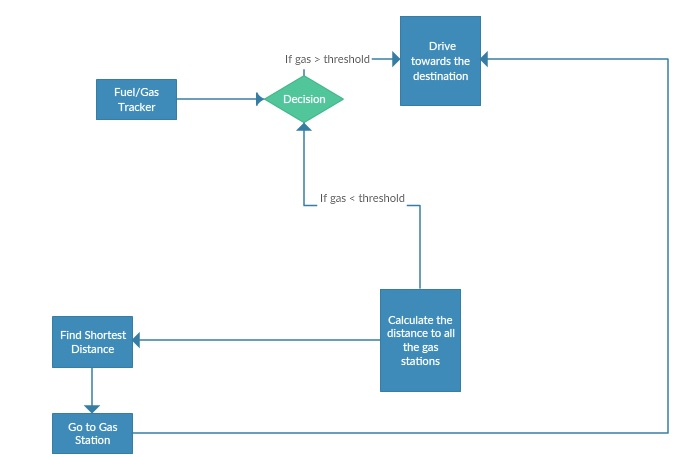
\includegraphics[width=1\columnwidth]{22}
  \end{center}
  \caption{\small Interactive model.}
  \label{fig-label}
\end{figure} \par

\subsection{Important Algorithms}
For our system, we have decided to use the popular A* algorithm to find the shortest path from the current location of the car to the destination..
A* is a best-first search, meaning that it solves problems by searching among all possible paths to the goal for the one that incurs the smallest cost (least distance travelled, shortest time, etc.), and among these paths it first considers the ones that appear to lead most quickly to the solution. It is formulated in terms of weighted graphs: starting from a specific node of a graph, it constructs a tree of paths starting from that node, expanding paths one step at a time, until one of its paths ends at the predetermined goal node.
At each iteration of its main loop, A* needs to determine which of its partial paths to expand into one or more longer paths. It does so on an estimate of the cost (total weight) still to go to the goal node. Specifically, A* selects the path that minimizes

\qquad\qquad\qquad\qquad\qquad F(n) = g(n) + h(n)

\noindent where n is the last node on the path, g(n) is the cost of the path from the start node to n, and h(n) is a heuristic that estimates the cost of the cheapest path from n to the goal. The heuristic is problem-specific. For our project we have decided to take the heuristic as the straight line distance to the goal.\\
\\
\noindent Pseudo Code:\\ 
OPEN: consists on nodes that have been visited but not expanded (meaning that successors have not been explored yet). This is the list of pending tasks.\\
CLOSE: consists on nodes that have been visited and expanded (successors have been explored already and included in the open list, if this was the case)\\
\begin{figure}[H]
  \begin{center}
    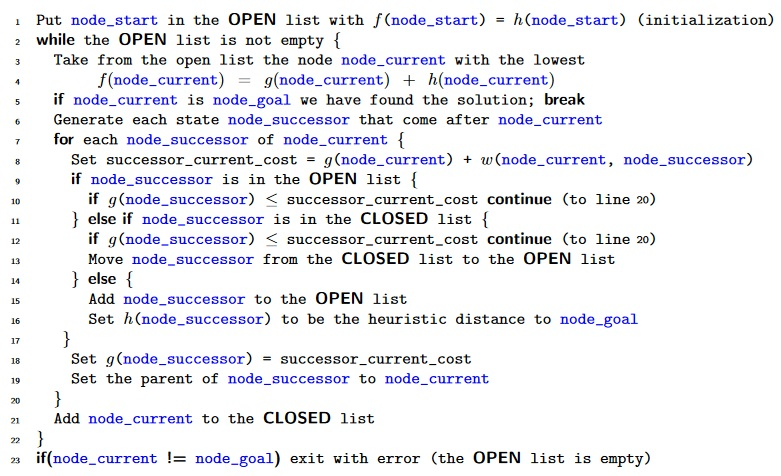
\includegraphics[width=1\columnwidth]{3}
  \end{center}
  \caption{\small A* pseudo code.}
  \label{fig-label}
\end{figure} \par

\section{Design and Test}
\subsection{Class Design}
Based on the above analysis, a class diagram of this project can be presented as following:\\

\begin{figure}[H]
  \begin{center}
    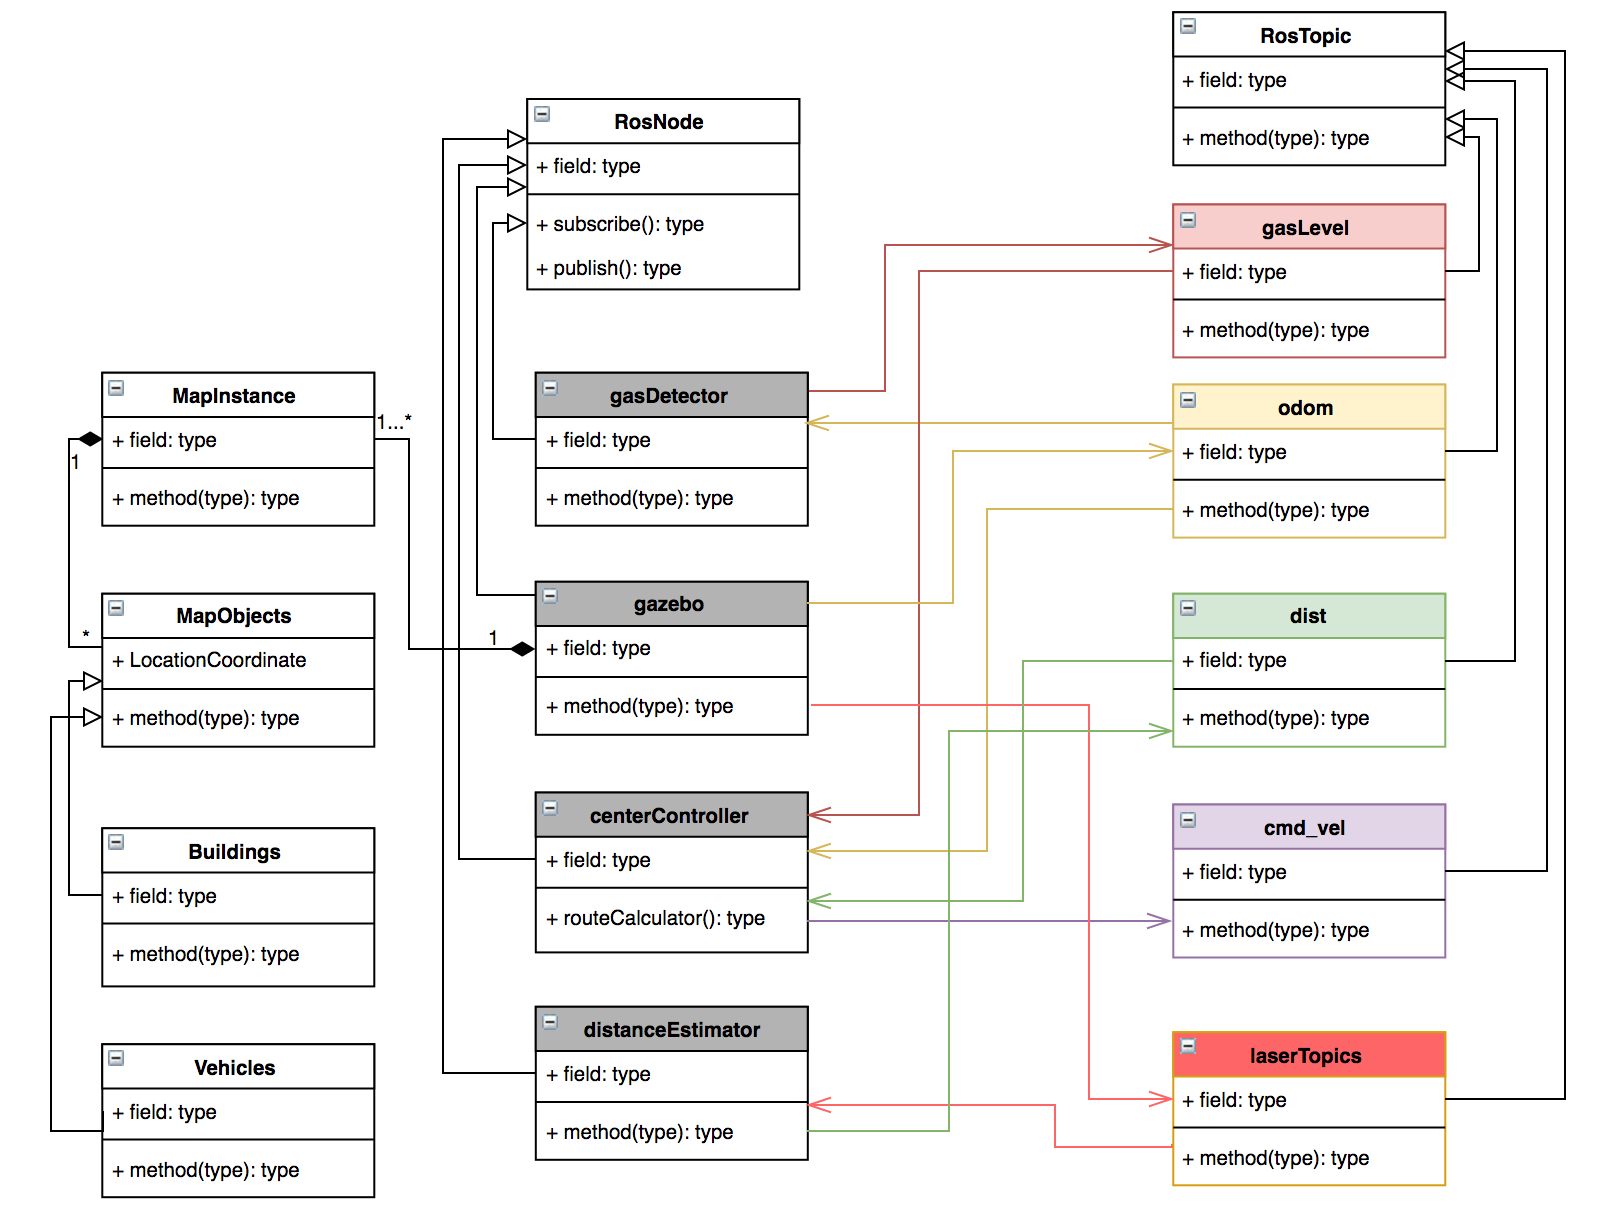
\includegraphics[width=1\columnwidth]{4}
  \end{center}
  \caption{\small Class Diagram.}
  \label{fig-label}
\end{figure} \par

\noindent Note that this is only the draft version of class diagram, most of the attribute and method for each class have not been defined but the basic associated relationship between Nodes and Topics have been demonstrated. \\
 
\noindent In the diagram, topic classes with the arrow connector at the end of association line means it is published by the counterpart node, vise visa, with arrow at node end means this topic is subscribed by this node. Most of nodes and topics that are not directly related to centerController and gazebo have been omitted due to the high complexity of the internal communication between them. Based on current project scope, two nodes and one topic will be created. GasDectector node is used to publish initial and real time gas level to centerController constantly via gasLevel topic. On the other hand, centerController is used to subscribe vehicle/gas station position data from gazebo node and obstacle's distance data from distanceEstimator node, via built-in topics odom and dist respectively, it then judges and calculates collected data by our core algorithm and publish proper result message to obstacleStopper (which is not showed in our class diagram) through cmd\_vel topic.\\ 
\\
\noindent In addition, this project's class design is based on below exception criteria and assumptions:\\
 
\noindent 
1. Some of the parameters in built-in node of catvehicle can be modified without any negative impact, such as the distanceEstimator.\\
2. Any reuses of existing topic will not cause any negative impact. \\
3. Messages subscribed from odom topic can be converted to coordinate data and distances data dynamically. \\
4. Gas stations' position data are predefined and known by centerController as parameters. \\
5. The coordinate proportion in the map instance is just to show how this project works, it does not reflect with the real world.\\
6. The gas consumption rate is just to show how this project works, it does not reflect with the real world.\\
7. The traffic condition and rules have been ignored to simplify the implementation.\\

\subsection{Testing Strategy}

\noindent The world file will be tested via gazebo to see if it meets every requirement and will be done by its creator. The gas detector node will be tested via gtest to check if it can publish messages to the certain topic and if the message is correct. The test will be done by its creator. The center control node will be tested via gtest.\\
 
\noindent First, we will check if each publisher and subscriber works(do they publish to or subscribe from right topics). It will be done by its creator. Then we will test the first and second algorithm via gtest. The first algorithm should tell us if the catvehicle needs to go to the gas station. We will copy it to the test file and provide different data like the value of the left gas and positions of gas stations and the catvehicle. The second algorithm should tell us which gas station is the closest one. Same as the first one, we provide different data and see if it can give us the result we expect. This test will be done by its creator.
The last algorithm should give proper commands to the catvehicle to drive it safely to the destination. To test it, we should pass all previous tests first and then do the simulation via gazebo. We will observe the behavior of the catvehicle and modify our works until they meet the requirement.

\subsection{Integration with Platform}

\noindent Based on current project scope, there is no direct interaction between our new-created nodes and vehicle's sensors in the map. The distance between vehicle and obstacles in the map is provided by front\_laser\_points topic and subscribed by distanceEstimator node through dist topic. By default, the only subscriber of this topic is obstacleStopper, now our centerController node will subscribe it as well in order to deal these data with our customized routing algorithm.\\
\\
\noindent On the other hand, given the high-complexity, instead of recognizing certain building objects in the map as gas station, we will set gas stations' position data as parameters of our centerController.

\section{Implementation Plan}
\subsection{Task allocation and breakdown}

The project will be divided into 4 tasks.\\
\\
\noindent Task1: create the world file\\
In the world file, there should be several gas stations in different position of the map. Also, there should be several obstacles between the catvehicle and each station to make the environment complex enough. The initial position of the catvehicle should be set in the world file, too.\\
\\
\noindent Task2: create the gas detector node\\
The gas detector node will publish the value of how much gas is left to a certain topic for the center control node. This value can be static or dynamic depending on the behavior of the catvehicle.\\
\\
\noindent Task3: create the frame of the center control node\\
The center control node should subscribe every position of gas stations in the map, the current position of the catvehicle and messages from the front sensor and the gas detector. Also it should publish proper messages to drive the catvehicle to the destination.\\ 
\\
\noindent Task4: write the algorithm of the center control node\\
There should be an algorithm in the center control node that figure out if the catvehicle should go to a gas station immediately, which depends on the messages from the gas detector and distances to each gas station. Also, another algorithm should provide proper commands to drive the catvehicle to the destination. The catvehicle should not hit any obstacle or go to other places instead of the destination.\\
\\
Task1 and Task2 will be done by Harish Kumar Kothari, Abhishek\\
Task3 will be done by Kejia Li\\
Task4 will be done by Zheng Li\\

\subsection{Timeline for Completion}

\begin{table}[H]
\centering
\begin{tabular}{|l|l|l|}
\hline
\rowcolor[HTML]{FFFC9E} 
\textbf{Date} & \textbf{Content of Work} & \textbf{Deliverable} \\ \hline
Week 10 & \begin{tabular}[c]{@{}l@{}}Each member complete the first version of their codes\\ and make them compiled\end{tabular} & Alpha release \\ \hline
Week 11 & \begin{tabular}[c]{@{}l@{}}Each member complete the first version of their codes\\ and make them compiled\end{tabular} &  \\ \hline
Week 12 & \begin{tabular}[c]{@{}l@{}}Start to do the simulation and modify codes until meet\\ requirements\end{tabular} &  \\ \hline
Week 13 & Release the beta version & Beta release \\ \hline
Week 14 & \begin{tabular}[c]{@{}l@{}}Get feedback from instructor and modify our work to\\ make it better\end{tabular} &  \\ \hline
Week 15 & \begin{tabular}[c]{@{}l@{}}Get feedback from instructor and modify our work to\\ make it better\end{tabular} & Final release \\ \hline
\end{tabular}
\caption{Timeline for Completion}
\label{my-label}
\end{table}

% this is a great place to put your table of abbreviations/acronyms
\newpage
\appendix





%\section{List of Acronyms and Abbreviations}


\newpage

%\bibliographystyle{abbrv}
%\bibliography{refs}
\end{document}
